\documentclass[12pt]{article}
\usepackage{listings}

\usepackage[T1]{fontenc}
\usepackage[utf8]{inputenc}
\usepackage{lmodern}
\usepackage{minted}
\usepackage{algpseudocode}
\usepackage{algorithm}
\usepackage{tikz} % Package for drawing
\usepackage{hyperref}

\title{Time Complexity Analysis of Trapezium Algorithm}
\author{Roy Ananth, Sambahangphe Mishek, Shea Jackson, Ng Sunnathan,\and and Desai Param}



\lstset{%
  basicstyle=\ttfamily,
  language=Java,
  showstringspaces=false,
  breaklines=true,
  frame=single,
  numbers=left
}

\begin{document}

\maketitle
\newpage
\section{Introduction}

Analysis of the trapezium algorithm in sequential and parallel forms has been tested with 100,000,000 partitions. The analysis shows that the sequential algorithm has a time complexity $\mathcal{O}(n)$ and the parallel algorithm has a time complexity of $\mathcal{O}(n)$. The parallel algorithm is faster because it is able to split the input n into sub threads and work on them simultaneously. The time complexity of the algorithms is the same. 

\section{Sequential Trapezium Algorithm}

\begin{minted}[mathescape, linenos, numbersep=5pt, gobble=0, frame=lines, framesep=2mm]{java} 
public static double trapezium(double a, double b, int n, FPFunction f) {
  double range = checkParamsGetRange(a, b, n);
  double nFloat = (double) n;
  double sum = 0.0;
  for (int i = 1; i < n; i++) {
    double x = a + range * (double) i / nFloat;
    sum += f.eval(x);
  }
  sum += (f.eval(a) + f.eval(b)) / 2.0;
  return sum * range / nFloat;
}
\end{minted}


\subsection{Hypothesis}
The sequential trapezium algorithm has a time complexity of $ \mathcal{O}(n)$. The main for loop iterates 'n' times where 'n' is the input size, while the other operations outside of the for loop have a time complexity of $\mathcal{O}(1) $, which is constant and does not depend on 'n'. Hence, the time complexity only depends on the for loop which will equate to $\mathcal{O}(n) + \mathcal{O}(1)$  = $\mathcal{O}(n)$ 




\newpage

\section{Parallel Trapezium Algorithm}


\begin{minted}[mathescape, linenos, numbersep=5pt, gobble=0, frame=lines, framesep=2mm]{java} 
public static double trapezium(double a, double b, int n, FPFunction f)
  {
    double range = checkParamsGetRange(a, b, n);

    return (IntStream.range(0, n).parallel().mapToDouble(i-> a + range * (double)i / n).map(x->f.eval(x)).sum()+ (f.eval(a) + f.eval(b)) / 2.0)* range / n;

  }
\end{minted}

\subsection{Hypothesis}
The parallel trapezium algorithm has a time complexity of $\mathcal{O}(n)$. Streams work the same as for-loops under the hood so the time complexity should be the same as a single for-loop, or $\mathcal{O}(n)$. The difference is that parallel streams can work simultaneously on the inputs by splitting into sub-threads. 

\section{Graph of Sequential Trapezium Algorithm}

\begin{center}
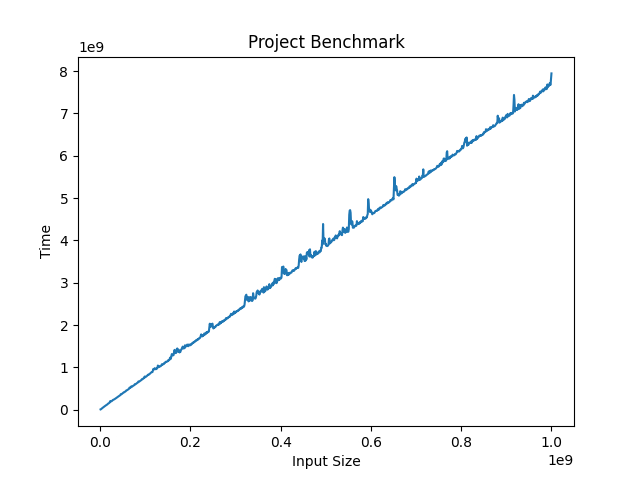
\includegraphics[width = 5in]{SequentialPlot.PNG}
\end{center}

\subsection{Analysis}
Our hypothesis that the sequential trapezium algorithm has a time complexity of $ \mathcal{O}(n)$ was correct. As n or input size grows the time required to complete the calculation increases linearly.  $ \mathcal{O}(n)$ increases linearly as the input size grows, therefore our hypothesis was correct. The sequential trapezium algorithm through analysis of the graph does indeed have a time complexity of $ \mathcal{O}(n)$.

\section{Graph of Parallel Trapezium Algorithm}

\begin{center}
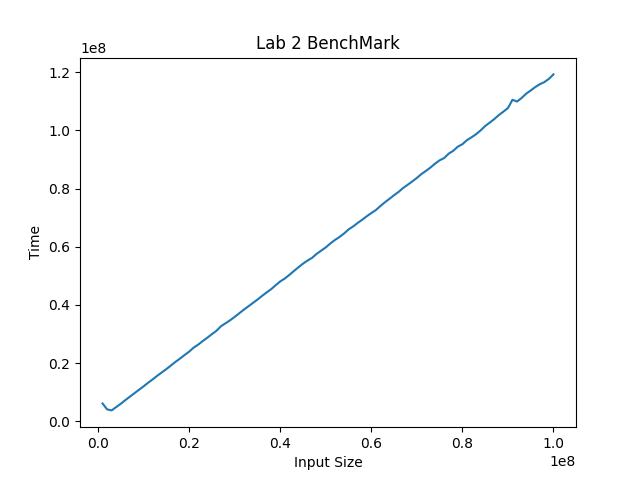
\includegraphics[width = 5in]{Parallelplot100.png}
\end{center}

\subsection{Analysis}
Our hypothesis that the parallel trapezium algorithm has a time complexity of $\mathcal{O}(n)$ was correct. As n or input size grows the time required to complete the calculation increases linearly.  $ \mathcal{O}(n)$ increases linearly as the input size grows, therefore our hypothesis was correct. The parallel trapezium algorithm through analysis of the graph does indeed have a time complexity of $ \mathcal{O}(n)$.

\newpage

\section{Conclusion}
Both the parallel and Sequential Trapezium algorithms have a time complexity of $ \mathcal{O}(n)$. Although they share the same time complexity, the parallel algorithm is faster because it is able to split the input n into sub threads and work on them simultaneously. When implementing the code, the sequential method is easier to understand but it is slower. The parallel method is faster but it is more difficult to understand.

\end{document}

